% =========================================================================== %

\begin{frame}[t,plain]
\titlepage
\end{frame}

% =========================================================================== %

\begin{frame}{Scope For Today}
%
\begin{itemize}
\item Fast Fourier Transform
	\begin{itemize}
	\item Some Math Recap
	\item SciPy's FFT API
	\item The Secret Behind JPEG
	\end{itemize}
\item Curve Fitting and Filters
	\begin{itemize}
	\item \texttt{scipy.optimize.curve\_fit}
	\item Method, Weaknesses and Remedies
	\item Detrending, Wiener Filter, Hipass/Lopass-Filter
	\end{itemize}
\item More cool stuff in SciPy
	\begin{itemize}
	\item Honorable Mentions
	\item Links to the docs
	\end{itemize}
\end{itemize}
%
\end{frame}

% =========================================================================== %

\begin{frame}{Fourier}
%
\begin{columns}
\column{.6\linewidth}
\begin{center}
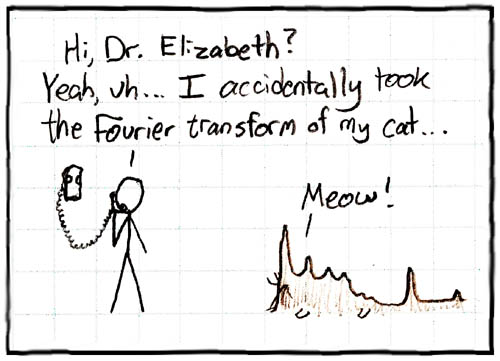
\includegraphics[width=\linewidth]{./gfx/05-xkcd-fourier}\\
\end{center}
%
\column{.2\linewidth}
\small
	\emph{That cat has some serious periodic components}

	\vspace{6pt}
	\url{https://xkcd.com/26/}
\end{columns}
%
\end{frame}

% =========================================================================== %

\begin{frame}{Definitions}
%
\begin{defbox}[Fourier-{,} Sine- and Cosine-Transformation]
\small
Fourier Transform
\begin{align*}
	\mathcal{F}_t[y](\omega)
=
	\hat{y}(\omega)
=
	\dfrac{1}{\mathcal{N}}	
	\int_{-\infty}^{\infty}
		y(t) \exp(-i\omega t) \dd{t}
&&
	\hat{y}: \mathbb{R} \to \mathbb{C}
\end{align*}

Fourier Cosine Transform
\begin{align*}
	\mathcal{F}^c_t[y](\omega)
=
	\hat{y}(\omega)
=
	\dfrac{1}{\mathcal{N}}
	\int_{-\infty}^{\infty}
		y(t) \cos(\omega t) \dd{t}
&&
	\hat{y}: \mathbb{R} \to \mathbb{R}
\end{align*}

Fourier Sine Transform
\begin{align*}
	\mathcal{F}^s_t[y](\omega)
=
	\hat{y}(\omega)
=
	\dfrac{1}{\mathcal{N}}
	\int_{-\infty}^{\infty}
		y(t) \sin(\omega t) \dd{t}
&&
	\hat{y}: \mathbb{R} \to \mathbb{R}
\end{align*}
\end{defbox}
%
\end{frame}

% =========================================================================== %

\begin{frame}{Refreshing Some Maths}
%
\begin{itemize}
\item Symmetry of Fourier Transform of real valued functions
	\begin{itemize}
	\item $\exp(i\omega t) \in \mathbb{C}$, in general.
	\item $\forall \omega, t \in \mathbb{R}: \exp(i\omega t) + \exp(-i\omega t)\in \mathbb{R}$
	\item Complex conjugate of products: $\overline{z_1 z_2} = \overline{z_1} \; \overline{z_2}$
	\item[\Thus] If $f(t): \mathbb{R} \to \mathbb{R}$ then
		\begin{itemize}
		\item For each frequency $\omega$, equal magnitude contribution of frequency $-\omega$
		\item Complex amplitude of $-\omega$ contribution is complex conjugate
		\item $\hat{f}(\omega) = a_\omega \exp(i\omega t) + \overline{a_\omega} \exp(-i\omega t)$
		\end{itemize}
	\end{itemize}
\item Inverse Transform
	\begin{itemize}
	\item Same integrals, but flip roles of $t$ and $\omega$
	\item Complex conjugate of basis: $\exp(-i\omega t) \to \exp(i\omega t)$
	\item Sine/Cosine Transform not affected
	\item Possibly different norm
	\end{itemize}
\end{itemize}
%
\end{frame}

% =========================================================================== %

\begin{frame}{Refreshing Some Maths}
%
\begin{itemize}
\item Normalization $\mathcal{N}$
	\begin{itemize}
	\setlength{\itemsep}{3pt}
	\item Depends on number of dimensions $n$
	\item Forward: $\mathcal{N}_{\text{transform}} = \dfrac{1}{(2\pi)^n}$, $\mathcal{N}_{\text{inverse}} = 1$
	\item Backward: $\mathcal{N}_{\text{transform}} = 1$, $\mathcal{N}_{\text{inverse}} = \dfrac{1}{(2\pi)^n}$
	\item Symmetric: $\mathcal{N}_{\text{transform}} = \dfrac{1}{(2\pi)^{\sfrac{n}{2}}}$, $\mathcal{N}_{\text{inverse}} = \dfrac{1}{(2\pi)^{\sfrac{n}{2}}}$
	\item Normalization factor comes from understanding Fourier Transform as scalar product
	\item Strictly speaking, only the forward definition makes sense
	\item Most of the time only interested in \emph{relative quantities}, so any normalization with 
	$\mathcal{N}_{\text{transform}} \cdot \mathcal{N}_{\text{inverse}} = \dfrac{1}{(2\pi)^n}$ will do
	\item Physicists very fond of the symmetric form because it reduces mental load
	\end{itemize}
\end{itemize}
%
\end{frame}

% =========================================================================== %

\begin{frame}{SciPy's FFT Package}
%
\begin{itemize}
\item One could use regular integration routines like \texttt{scipy.integrate.quad}
	\begin{itemize}
	\item Each integration: $\mathcal{O}(N)$
	\item Need to redo for \emph{multiple} values of $\omega$
	\item[\Thus] $\mathcal{O}(N^2)$
	\end{itemize}
\item \emph{Fast} Fourier Transform
	\begin{itemize}
	\item Realize: Some products $f(t) \exp(-i\omega t)$ appear in multiple integrals because of periodicity of $\exp(it)$
	\item Highest efficiency for $f \in \mathbb{R}^{2^k}$
	\item Exploiting this allows to get to $\mathcal{O}(N \log(N))$
	\item Condition: $\Delta t = \text{const}$
	\end{itemize}
\item Functions in \texttt{scipy.fft}
	\begin{itemize}
	\item \texttt{fft} -- Discrete Fourier Transform, complex valued
	\item \texttt{dst} and \texttt{dct} -- Discrete Sine/Cosine Transform, real valued
	\item \texttt{fft2}, \texttt{fftn}, \texttt{dctn}, \texttt{dstn} -- 2-dimensional and $N$-dimensional transforms
	\item \texttt{ifft}, \texttt{ifft2}, ... -- inverse transforms
	\end{itemize}
\end{itemize}
%
\end{frame}

% =========================================================================== %

\begin{frame}{\texttt{scipy.fft.fft}}
%
\begin{itemize}
\item One mandatory parameter
	\begin{itemize}
	\item Function to transform, as precomputed array of length $N$
	\item Equidistant evaluation: \texttt{f[k]} = $f(t_k) = f(k \Delta t)$
	\end{itemize}
\item Many optional parameters
	\begin{itemize}
	\item \texttt{norm}: Either of \inPy{'forward'}, \inPy{'backward'}, \inPy{'ortho'}\\
		Default: \inPy{'backward'}
	\item \texttt{axis}: When passing a multidimensional array, do multiple transforms at once.\\
		Default: \inPy{axis=-1}
	\end{itemize}
\item Returns array
	\begin{itemize}
	\item Function in frequency domain, complex valued
	\item \inPy{result[0]}: constant offset (frequency = 0)
	\item \inPy{result[k]} for $\texttt{k} \in [1, ..., \lfloor \sfrac{N}{2} \rfloor]$: complex amplitude for $\omega = \dfrac{2\pi k}{\max(t_k)}$
	\item \inPy{result[k]} for $\texttt{k} \in [\lfloor \sfrac{N}{2} \rfloor + 1, ... N -1]$: complex amplitude for $\omega = \dfrac{2\pi (k-N)}{\max(t_k)}$
	\item[\Thus] Shifted by $\sfrac{N}{2}$. Undo with \texttt{np.roll(result, N//2)} or use \texttt{scipy.fft.fftshift}
	\end{itemize}
\end{itemize}
%
\end{frame}

% =========================================================================== %

\begin{frame}[fragile]
%
\begin{codebox}[1D Fourier Transform]
\begin{minted}[linenos, fontsize=\scriptsize]{python3}
N = 200
frequency_1 = 3
amplitude_1 = 2
frequency_2 = 20
amplitude_2 = 1

xs = np.linspace(0, 2 * np.pi, N)
ys = amplitude_1 * np.sin(frequency_1 * xs) + amplitude_2 * np.cos(frequency_2 * xs)

frequencies = 2 * np.pi * np.arange(-N//2, +N//2) / xs[-1]

fft = scipy.fft.fft(ys)
fft = np.roll(fft, N//2)
# these two lines could be combined into fft = scipy.fft.fftshift(ys)

# (plus matplotlib code)
\end{minted}
\end{codebox}
%
\end{frame}

% =========================================================================== %

\begin{frame}{Output: 1D Fourier Transform}
%
\begin{columns}
\column{.6\linewidth}
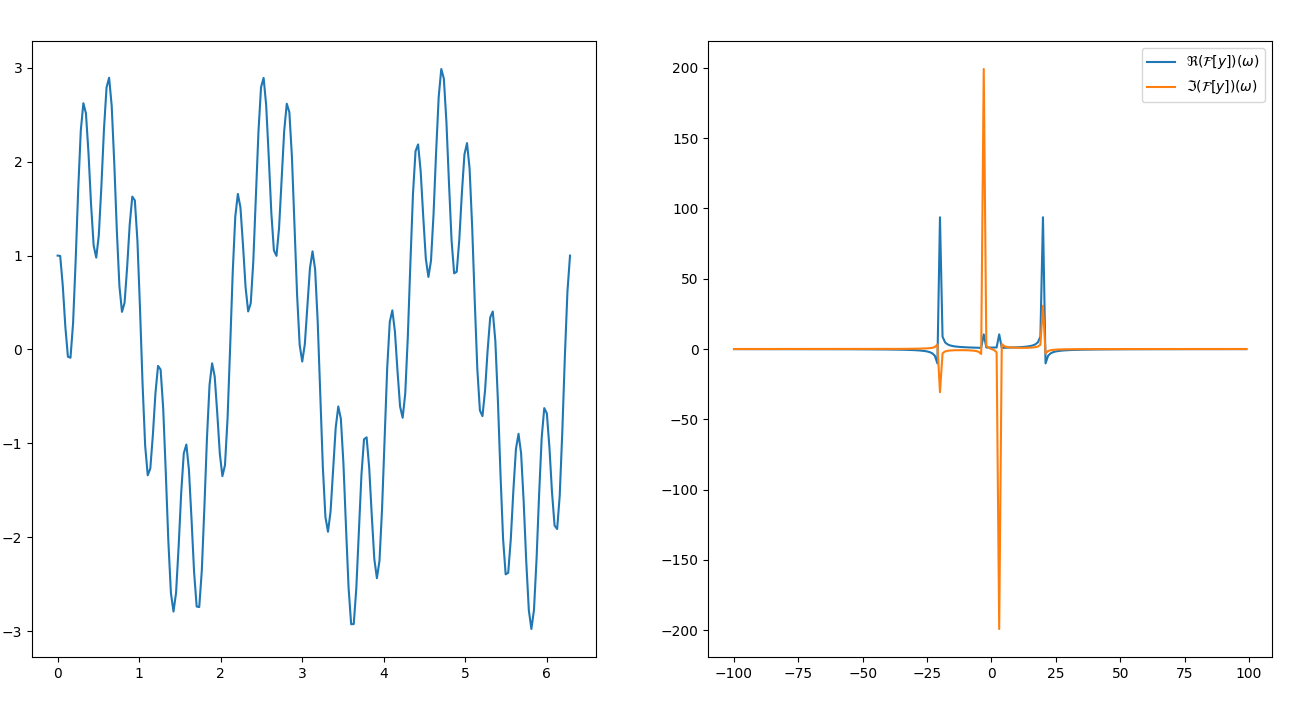
\includegraphics[width=\linewidth]{./gfx/05-FFT-1D}
%
\column{.35\linewidth}
\begin{itemize}
\item Note the numerical artefacts
	\begin{itemize}
	\item Non-zero real component of sine component
	\item Non-zero imaginary component of cosine component
	\item Peak width greater than $\Delta \omega$
	\end{itemize}
\end{itemize}
\end{columns}
%
\begin{hintbox}[Resolution and Width of Spectrum]
\footnotesize
The spectral resolution depends inversely on the length $t_{\text{max}}$ of signal.\\
The maximum frequency in the spectrum is given by the number of data points $N$ of signal.
\end{hintbox}
%
\end{frame}

% =========================================================================== %

\begin{frame}{Definitions}
%
\begin{defbox}[Multi-Dimensional Fourier Transform]
\small
Fourier Transform
\begin{align*}
	\mathcal{F}_{\vec{r}}[y](\vec{k})
=
	\hat{y}(\vec{k})
=
	\dfrac{1}{\mathcal{N}_{\text{transform}}}	
	\int_{\mathbb{R}^n}
		y(\vec{r}) \exp(-i\vec{k} \cdot \vec{r}) \dd[n]{\vec{r}}
&&
	\hat{y}: \mathbb{R}^{n} \to \mathbb{C}
\end{align*}


Inverse Fourier Transform
\begin{align*}
	\mathcal{F}_{\vec{k}}^{-1}[\hat{y}](\vec{k})
=
	y(\vec{r})
=
	\dfrac{1}{\mathcal{N}_{\text{inverse}}}	
	\int_{\mathbb{R}^n}
		y(\vec{r}) \exp(+i\vec{k} \cdot \vec{r}) \dd[n]{\vec{k}}
&&
	\hat{y}: \mathbb{R}^{n} \to \mathbb{C}
\end{align*}

And likewise for Sine- and Cosine-Transform.
\end{defbox}
%
\end{frame}

% =========================================================================== %

\begin{frame}[fragile]
%
\begin{codebox}[2D Fourier Transform And The Secret Of JPEG]
\begin{minted}[linenos, fontsize=\scriptsize]{python3}
# example picture for quick tests, built into scipy
img_original = 256 - sci.misc.ascent()
fft_original = sci.fft.fft2(img_original)

# for plotting:
# compute absolute values from complex Fourier data
# low-frequency contributions are dominant. Compute log to bring them closer together
display_original = roll(np.log(np.absolute(fft_original)))

img_size = img_original.shape
mask = create_cirular_mask(img_size, 20)
    
fft_hi_pass_filter = roll(fft_original.copy())
fft_hi_pass_filter[mask] = 0
display_hi_pass_filter = roll(np.log(np.absolute(fft_hi_pass_filter)))
fft_hi_pass_filter = roll(fft_hi_pass_filter)
img_hi_pass_filter = sci.fft.ifft2(fft_hi_pass_filter).real
display_hi_pass_filter = roll(display_hi_pass_filter)

# similar for low pass filter
# matplotlib-commands
\end{minted}
\end{codebox}
%
\end{frame}

% =========================================================================== %

\begin{frame}{2D Fourier Transform And The Secret Of JPEG}
%
\begin{columns}[T]
\column{.75\linewidth}
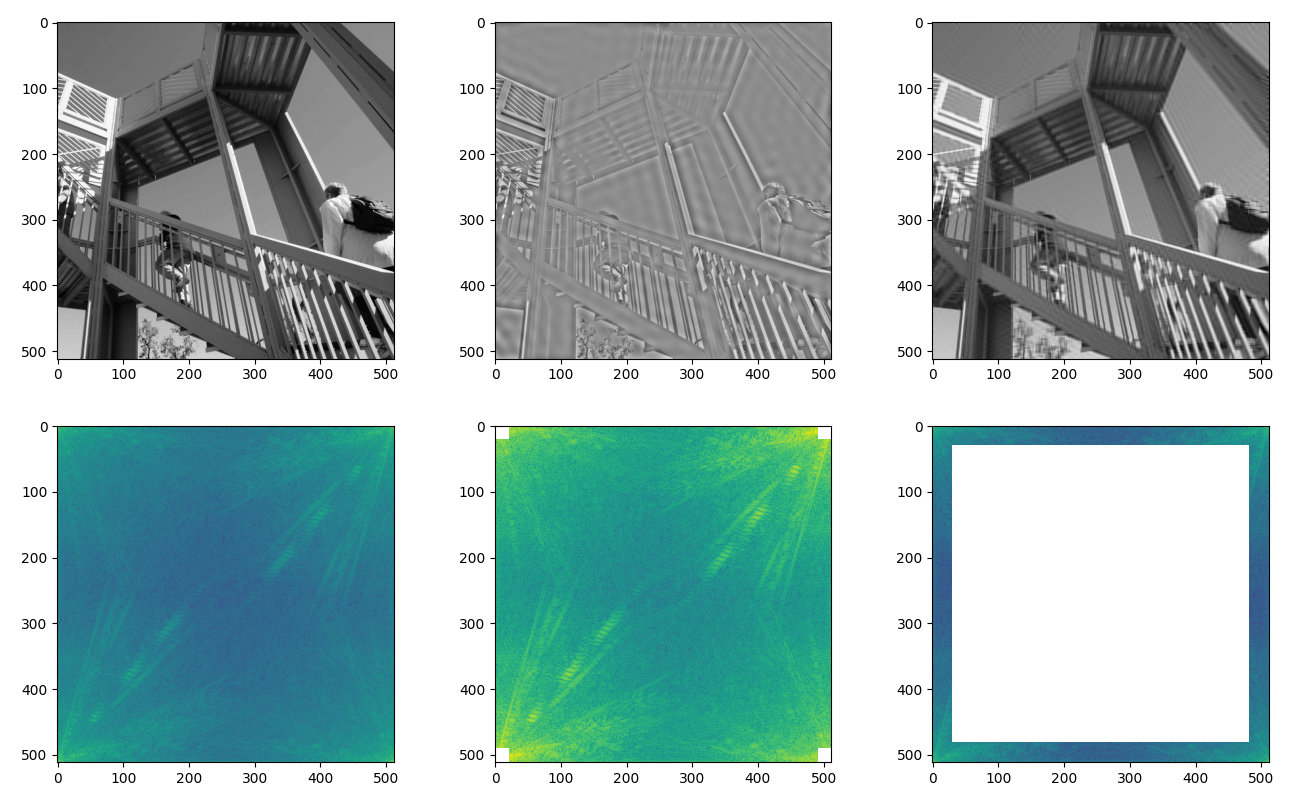
\includegraphics[width=\linewidth]{./gfx/05-FFT-2D}
%
\column{.2\linewidth}
\begin{itemize}
\item Largest part of spectrum: negligible
\item Remove high frequency components 
\item[\Thus] Deterioration of picture quality, but not very much
\end{itemize}
\end{columns}
%
\end{frame}

% =========================================================================== %

\begin{frame}{Curve-Fitting}
%
\vspace{-12pt}
\begin{columns}[T]
\column{.5\linewidth}
\begin{center}
	\vspace{60pt}
	\emph{Cauchy-Lorentz: \enquote{Something alarmingly mathematical is happening, and you should probably pause to Google my name and check what field I originally worked in.}}

	\vspace{6pt}
	Source: \url{https://xkcd.com/2048/}
\end{center}
%
\column{.5\linewidth}
\vspace{-43pt}
\begin{center}
	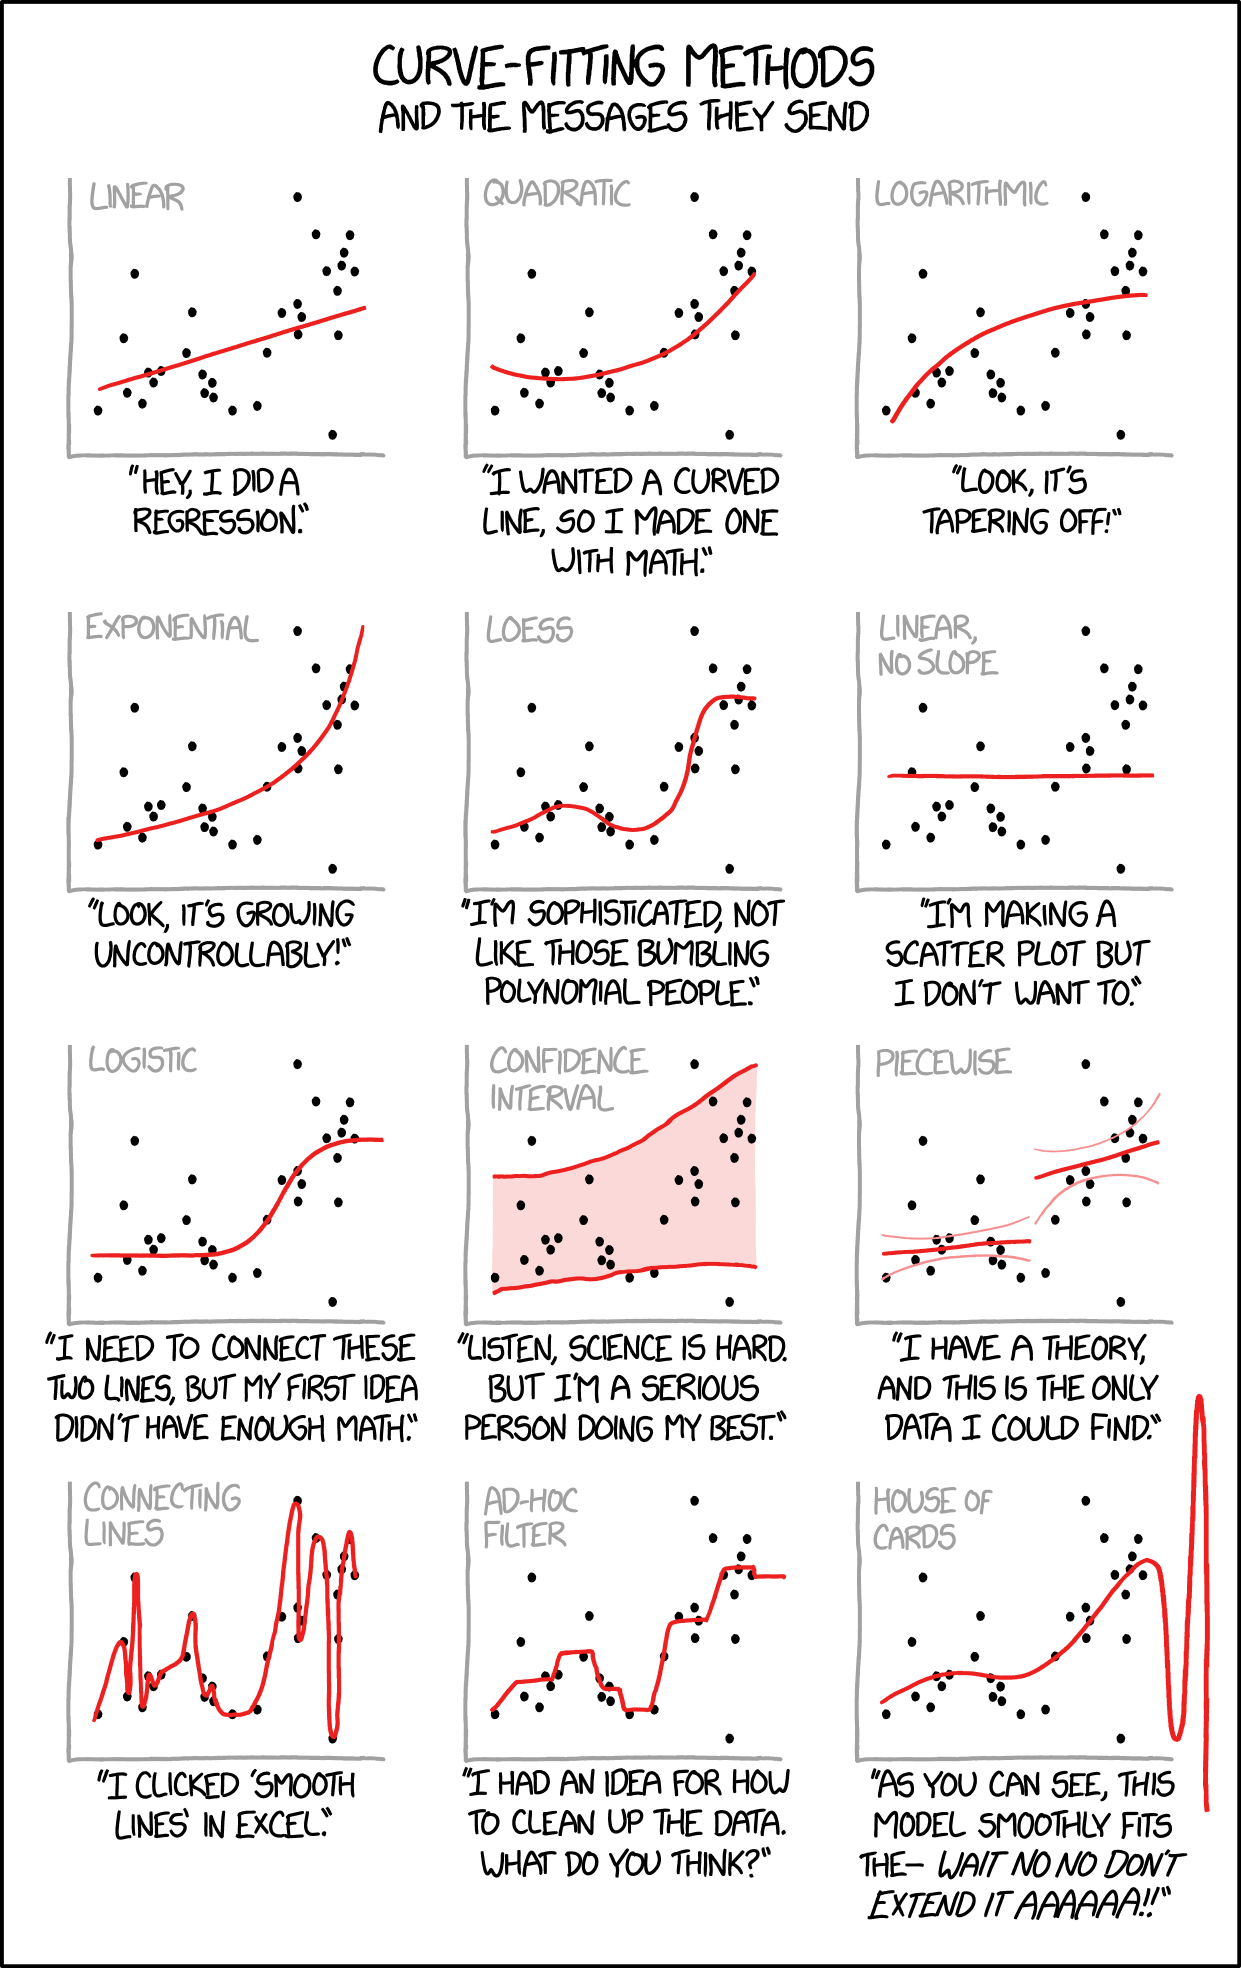
\includegraphics[width=.74\linewidth]{./gfx/05-xkcd-curveFitting}
\end{center}
\end{columns}
%
\end{frame}

% =========================================================================== %

\begin{frame}{\texttt{scipy.optimize.curve\_fit}}
%
\begin{itemize}
\item Reconstruct analytical formula from given data
\item Or better: find parameters for a given curve form
	\begin{itemize}
	\item E.\;g. $f(x) = ax^2 + bx + c$ \Thus find $a, b, c$
	\end{itemize}
\item Minimal form: \texttt{curve\_fit(f, xs, ys)}
	\begin{itemize}
	\item \texttt{f}: Callable with 1 + N arguments
		\begin{itemize}
		\item 1$^{\text{st}}$ argument is $x$
		\item Arguments $2 ... N+1$ are paramters $a, b, ...$
		\end{itemize}
	\item \texttt{xs}, \texttt{ys}: 1D-sequences of x/y values
	\item Return value: \inPy{tuple (popt, pcov)}
		\begin{itemize}
		\item \texttt{popt}: parameters $a, b, ...$ as \inPy{tuple}
		\item \texttt{pcov}: covariance matrix as \texttt{numpy.ndarray}\\
			Square root of diagonal elements gives standard deviation of respective parameters
		\end{itemize}
	\end{itemize}
\end{itemize}
%
\end{frame}

% =========================================================================== %

\begin{frame}[fragile]
%
\begin{codebox}[Simple Call To \texttt{curve\_fit}]
\begin{minted}[linenos, fontsize=\scriptsize]{python3}
res = 250
amplitude = 1
decay = 5
amplitude_noise = 0.1

f = lambda x, a, k : a * np.exp(-k * x)

xs = np.linspace(0, 1, res)
ys = f(xs, amplitude, decay) + amplitude_noise * np.random.random(res)

popt, pcov = scipy.optimize.curve_fit(f, xs, ys)
reconstructed = f(xs, *popt)

print(pcov)
print(np.sqrt(np.diag(pcov)))

plt.plot(xs, ys, label="signal")
plt.plot(xs, reconstructed, label="{0:4.2f} $\\exp(-${1:4.2f}$t)$".format(*popt))
plt.legend()
plt.show()
\end{minted}
\end{codebox}
%
\end{frame}

% =========================================================================== %

\begin{frame}[fragile]{Result: Simple Call To \texttt{curve\_fit}}
%
\begin{columns}
\column{.45\linewidth}
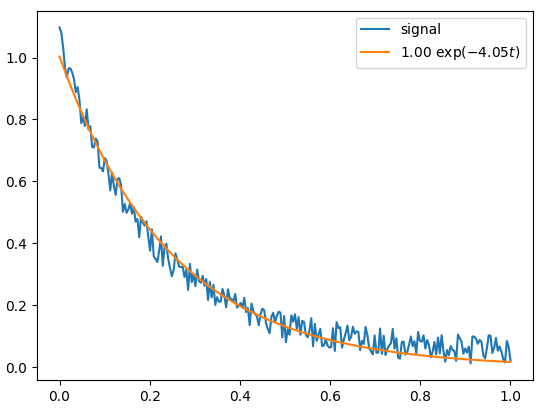
\includegraphics[width=\linewidth]{./gfx/05-simple-fit}
%
\column{.5\linewidth}
\begin{cmdbox}[Output: Simple Call To \texttt{curve\_fit}]
\begin{minted}[fontsize=\scriptsize]{text}
[[8.95725524e-05 3.65483288e-04]
 [3.65483288e-04 3.00940484e-03]]
[0.00946428 0.05485804]
\end{minted}
\end{cmdbox}
%
\begin{itemize}
\item Signal/Noise Ratio (SNR) bad \Thus bad fit
	\vspace{-12pt}
	\begin{itemize}
	\item \inPy{decay = 5}, but \inPy{decay_fit = 4.05}
	\item Covariance matrix does not hint at this
	\end{itemize}
\item Still, overall okay result
\end{itemize}
\end{columns}
%
\end{frame}

% =========================================================================== %

\begin{frame}{How Does It Do That?}
%
\begin{itemize}
\item Start with an initial guess \inPy{p0 = (1, 1, ...)}
\item Compute error function \inPy{err = np.sum( (ys - f(xs, *p0))**2 )}
\item Minimize error function with \emph{Trust Region Reflective} and update $p^{(n)} \to p^{(n+1)}$
	\begin{itemize}
	\item Assumes $\mathcal{C}^{1}$ function
	\item Essentially refinement of Newton Root finding method
		\begin{itemize}
		\item Repeatedly compute tangents to graph in $p^{(n)}$
		\item Find Zeros of tangents \Thus $p^{(n+1)}$
		\end{itemize}
	\end{itemize}
\item Other algorithms available
	\begin{itemize}
	\item Optional parameter \texttt{method}
	\item Search for \emph{dogleg algorithm} and \emph{Levenberg-Marquardt algorithm}
	\end{itemize}
\end{itemize}
%
\begin{hintbox}[Providing Initial Guesses]
\small
With the optional parameter \texttt{p0 = tuple\_of\_initial\_guesses} you can improve both, the accuracy and runtime behaviour of \texttt{curve\_fit}.
\end{hintbox}
%
\end{frame}

% =========================================================================== %

\begin{frame}{Tangent: \texttt{scipy.optimize.least\_squares}}
%
\begin{itemize}
\item Generic Method to find $x_{\text{min}} = \arg\min{f(x)}$
	\begin{itemize}
	\item $x_{\text{min}} \in \mathbb{R}^{N}$
	\item $f: \mathbb{R}^{n} \to \mathbb{R}^{m}$
	\end{itemize}
\item Used by \texttt{curve\_fit}
\item Returns \texttt{OptimizeResult} object with several attributes
	\begin{itemize}
	\item \texttt{x} -- $x_{\text{min}}$
	\item \texttt{fun} -- $f(x_{\text{min}})$
	\item \texttt{cost} -- value of the error function in $x_{\text{min}}$
	\end{itemize}
\end{itemize}
%
\begin{hintbox}[See the online docs]
\small
Details can be found here:
\url{https://docs.scipy.org/doc/scipy/reference/generated/scipy.optimize.least_squares.html}
\end{hintbox}
%
\end{frame}

% =========================================================================== %

\begin{frame}{Weaknesses and Remedies}
%
\begin{itemize}
\item Order of magnitude
	\begin{itemize}
	\item When parameters very small or very big compared to 1: premature termination of optimization
	\item[\Thus] \emph{Always} use \texttt{p0}, to provide at least proper power of 10
	\end{itemize}
\item SNR/Small values
	\begin{itemize}
	\item[\Thus] Try Noise Filters
		\begin{itemize}
		\item See in a couple of slides
		\end{itemize}
	\item[\Thus] Only use values where SNR sufficiently high
		\begin{itemize}
		\item Filter using a mask
		\item \texttt{mask = signal > threshold}
		\item \texttt{xs\_for\_fit = xs[mask]}; analogous for \texttt{signal}
		\end{itemize}
	\end{itemize}
\item Periodic Functions (with more than one repetition)
	\begin{itemize}
	\item[\Thus] Use a mask that selects only one oscillation
	\end{itemize}
\end{itemize}
%
\end{frame}

% =========================================================================== %

\begin{frame}[fragile]
%
\begin{codebox}[Problems With Periods]
\begin{minted}[linenos, fontsize=\scriptsize]{python3}
tau = 2 * np.pi
res = 250
amplitude_true = 3
frequency_true = 7 * tau
f = lambda t, amplitude, frequency: amplitude * np.sin(frequency * t)

xs = np.linspace(0, 1, res)
ys = f(xs, amplitude_true, frequency_true)

window = slice(0, 20, 1)

popt_naive, pcov_naive = scipy.optimize.curve_fit(f, xs, ys)
popt_hint, pcov_hint = scipy.optimize.curve_fit(f, xs, ys, p0=(5, 20))
popt_window, pcov_window = scipy.optimize.curve_fit(f, xs[window], ys[window])

# printing table with standard deviations
# matplotlib code
\end{minted}
\end{codebox}
%
\end{frame}

% =========================================================================== %

\begin{frame}[fragile]{Result: Problems With Periods}
%
\begin{columns}
\column{.45\linewidth}
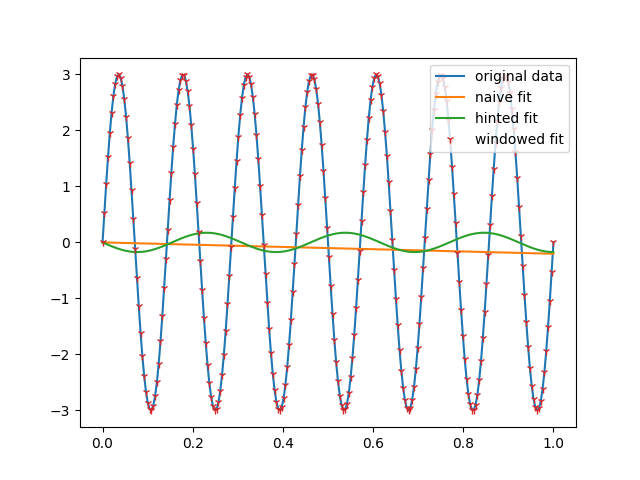
\includegraphics[width=\linewidth]{./gfx/05-curvefit-fail}
%
\column{.5\linewidth}
\begin{cmdbox}[Output: Problems With Periods]
\begin{minted}[fontsize=\scriptsize]{text}
method     amplitude           frequency
naive  -11.030 ± 405626.0  +0.018 ± 699.58
hinted  -0.173 ±      0.2 +20.423 ±   1.91
window  +3.000 ±      0.0 +43.982 ±   0.00
\end{minted}
\end{cmdbox}
\end{columns}
%
\end{frame}

% =========================================================================== %

\begin{frame}{Fitting Multivariate Functions}
%
\begin{itemize}
\item Assume $f = f(x, p); x \in \mathbb{R}^{n}, p \in \mathbb{R}^{m}$
\item Cannot directly use \texttt{curve\_fit}, as it expects $x \in \mathbb{R}$
\item But: we can provide set of functions $f_i(t, p) = \eval{f(x, p)}_{x_i = t}$
	\begin{itemize}
	\item Sneak Peek: \texttt{functools.partial} can do exactly that
	\end{itemize}
\item Fit $f_1$ and use obtained $p$ as initial guess for fitting $f_2$; iterate
\end{itemize}
%
\begin{warnbox}[Instable Method]
\small
Use this approach only as a last resort and always double check if your fit at least makes sense!\\
See GRIPS for a 2D example.
\end{warnbox}
%
\end{frame}

% =========================================================================== %

\begin{frame}{Tangent: Runge Spikes}
%
\begin{columns}
\column{.5\linewidth}
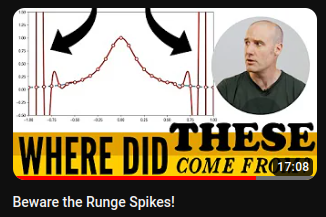
\includegraphics[width=.8\linewidth]{./gfx/05-runge-spikes}
\url{https://youtu.be/F_43oTnTXiw}
%
\column{.4\linewidth}
\begin{itemize}
\item You can perfectly fit a polynomial of degree $N$ on $N + 1$ data points
\item The result does not necessarily make sense
\item Only fit functions that actually make sense in the context
\item If you do use polynomials as an approximation, use Chebyshev spacing
\end{itemize}
\end{columns}
%
\end{frame}

% =========================================================================== %

\begin{frame}{Metamaterials}
%
\begin{columns}
\column{.6\linewidth}
\begin{center}
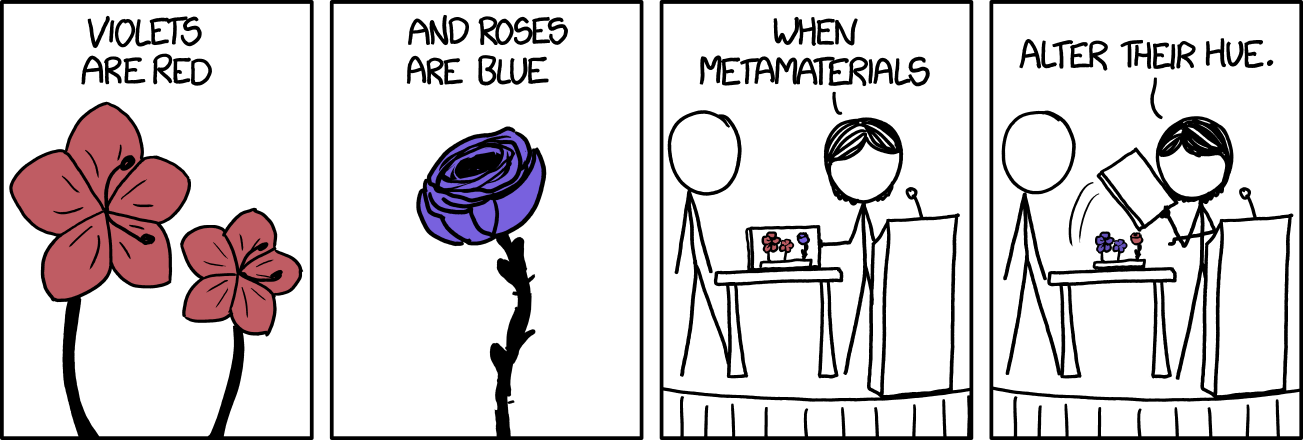
\includegraphics[width=\linewidth]{./gfx/05-xkcd-metamaterials}\\
\end{center}
%
\column{.3\linewidth}
\small
	\emph{If I developed a hue-shifting metamaterial, I would photobomb people's Instagram pics with a sheet of material that precisely undid the filter they were using.}

	\vspace{6pt}
	\url{https://xkcd.com/1351/}
\end{columns}
%
\end{frame}

% =========================================================================== %

\begin{frame}{Noise Filters}
%
\begin{itemize}
\item Assumption: $y(t) = f(t) + n(t)$
	\begin{itemize}
	\item $y(t)$: Recorded signal
	\item $f(t)$: \enquote{true}, physical principle
	\item $n(t)$: Noise
	\end{itemize}
\item Systematic error
	\begin{itemize}
	\item Constant offset
	\item Linear trend
	\item ...
	\end{itemize}
\item Random noise
	\begin{itemize}
	\item Average zero
	\item Uniform or symmetric distribution (\zB Gaussian) around zero
	\end{itemize}
\item Combination of both
\end{itemize}
%
\end{frame}

% =========================================================================== %

\begin{frame}{Removing Systematic Error: \texttt{scipy.signal.detrend}}
%
\begin{itemize}
\item Determines a linear trend of form $n(t) = s \cdot t + o$
	\begin{itemize}
	\item $o$: constant offset, $o = \dfrac{1}{N} \sum_i y_i$
	\item $s$: average slope, such that $\sum_i y_i - o - s \cdot i = 0$
	\item[\Thus] Assumption: Equidistant data points
	\end{itemize}
\item Usage
	\begin{itemize}
	\item Most simple: \\
		\texttt{f = detrend(y)}
	\item Constant offset only: \\
		\texttt{f = detrend(y, type='constant')}
	\item Multiple series at once: \\
		\texttt{f = detrend(y, axis=...)}
	\item Multiple regions with different offset/slope: \\
		\texttt{f = detrend(y, bp=[t\_on, t\_off, ...])}
	\end{itemize}
\end{itemize}
%
\end{frame}

% =========================================================================== %

\begin{frame}{Removing Random Noise: Gliding Average}
%
\begin{itemize}
\item Use assumption: average of noise is zero
\item Convolve with $
	\sfrac{1}{W} 
	\underbrace{
	\begin{pmatrix}
	1 & 1 & \ldots & 1
	\end{pmatrix}
	}_{W \text{ times}}
	$
\item Alternative: Gaussian Filter: Convolve with $\sfrac{1}{\mathcal{N}} G$
	\begin{itemize}
	\item $G \in \mathbb{R}^{1 \times W}$
	\item $G_k = \exp[-(k - \lfloor\sfrac{W}{2}\rfloor)^2]$
	\item $\mathcal{N} = \sum_k G_k$
	\item Better perservation of peaks than unweighted average
	\end{itemize}
\item Alternative: Median Filter
	\begin{itemize}
	\item Pick the median value in a window of width $W$
	\item Introduces no new values to the dataset
	\item Ready implemented: \texttt{scipy.signal.medfilt} and \texttt{scipy.signal.medfilt2d}
	\end{itemize}
\end{itemize}
%
\end{frame}

% =========================================================================== %

\begin{frame}{Removing Random Noise II: Electric Boogaloo}
%
\begin{itemize}
\item Wiener Filter
	\begin{itemize}
	\item Adaptive convolution kernel: $G_k$ depend on \enquote{last seen} $y_k$
	\item Ready implemented: \texttt{scipy.signal.wiener} 
	\end{itemize}
\item Savitzky–Golay Filter
	\begin{itemize}
	\item Assumption: $f(t)$ is locally a polynomial of degree $n$
	\item Compute convolution kernel of width $W$ that gives best fit through dataset
	\item Ready implemented: \texttt{scipy.signal.savgol\_filter} 
	\end{itemize}
\item Fourier Hipass/Lopass Filter
	\begin{itemize}
	\item Assumption: Random noise introduces high frequency oscillation
	\item Trends introduce low frequency components
	\item[\Thus] Selectively set parts of Fourier Spectrum to 0 and recompute the signal
	\end{itemize}
\end{itemize}
%
\end{frame}

% =========================================================================== %

\begin{frame}{Filtered Signals -- Examples}
%
\begin{columns}
\column{.7\linewidth}
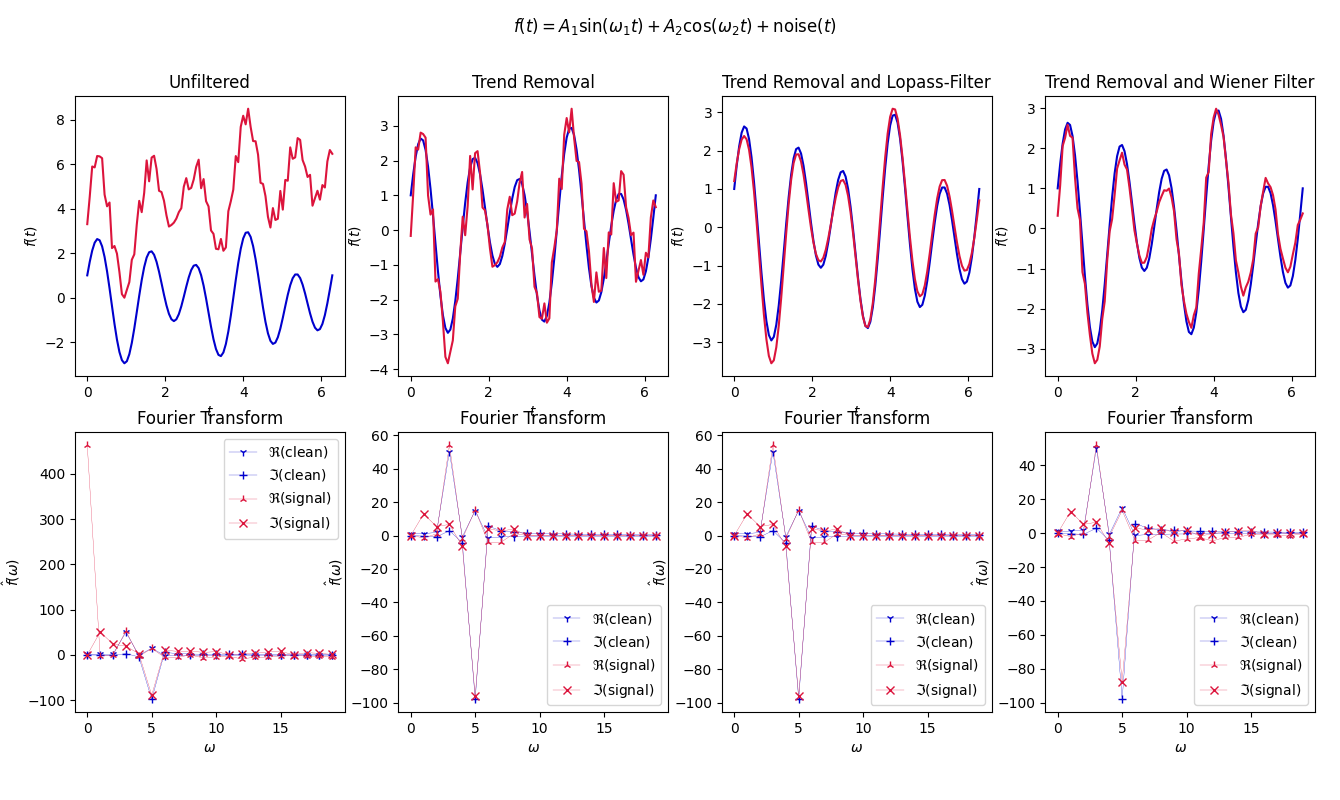
\includegraphics[width=\linewidth]{./gfx/05-filters}
%
\column{.3\linewidth}
\begin{hintbox}[Which Filter to Use]
\footnotesize
There is no really good answer. None of the filters work well with discontinuities (apply piecewise filters if you know there's a jump). All have a tendency to flatten peaks.\\
Toy around to see what suits you best. In doubt, use the most simple filter to reduce complexity and computation time.
\end{hintbox}
\end{columns}
%
\end{frame}

% =========================================================================== %

\begin{frame}{Everything}
%
\begin{columns}
\column{.6\linewidth}
\begin{center}
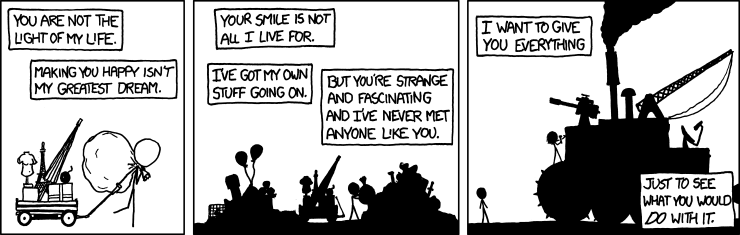
\includegraphics[width=\linewidth]{./gfx/05-xkcd-everything}\\
\end{center}
%
\column{.3\linewidth}
\small
	\emph{I wanna hold your hand so I don't fall out of your gyrocopter.}

	\vspace{6pt}
	\url{https://xkcd.com/968/}
\end{columns}
%
\end{frame}

% =========================================================================== %

\begin{frame}[fragile]{Constants}
%
\vspace{-4pt}
\begin{columns}[T]
\column{.5\linewidth}
\begin{itemize}
\item Direct access
	\begin{itemize}
	\item \texttt{scipy.pi}
	\item \texttt{scipy.constants.golden}\\
	 (golden ratio, $\frac{1 + \sqrt{5}}{2} \approx 1.618$)
	\item \texttt{scipy.constants.c}, \texttt{scipy.constants.h}, \texttt{scipy.constants.hbar}, ...
	\item SI units
	\end{itemize}
\item Access via functions
	\begin{itemize}
	\item \texttt{scipy.constants.value}: numerical value
	\item \texttt{scipy.constants.unit}: physical dimension as string
	\item \texttt{scipy.constants.precision}: relative error of numerical value
	\end{itemize}
\end{itemize}
%
\column{.5\linewidth}
\begin{codebox}[Example: SciPy Constants]
\begin{minted}[fontsize=\scriptsize]{python3}
print(sc.pi)
print(
  sc.value    ('Avogadro constant'), "±",
  sc.precision('Avogadro constant'),
  sc.unit     ('Avogadro constant'))
print()
\end{minted}
\end{codebox}
%
\begin{cmdbox}[Output: SciPy Constants]
\begin{minted}[fontsize=\scriptsize]{text}
3.141592653589793
6.02214076e+23 ± 0.0 mol^-1
\end{minted}
\end{cmdbox}
%
See Documentation\\
	\scriptsize \url{https://docs.scipy.org/doc/scipy/reference/constants.html}
\end{columns}
%
\end{frame}

% =========================================================================== %

\begin{frame}[fragile]
%
\begin{columns}[T]
\column{.5\linewidth}
\begin{Large}
	{Special Functions}
	\vspace{6pt}
\end{Large}
%
\begin{itemize}
\item \emph{Huge} collection of (more or less) common functions
	\begin{itemize}
	\item Airy functions
	\item Elliptic functions and integrals
	\item Bessel functions
		\begin{itemize}
		\item Zeros of Bessel functions
		\item Integrals of Bessel functions
		\item Derivatives of Bessel functions
		\item Spherical Bessel functions
		\item Riccati-Bessel functions
		\end{itemize}
	\item Struve functions
	\item Raw statistical functions
	\item Information Theory functions
	\item Gamma and related functions
	\item Error function and Fresnel integrals
	\item Legendre functions
	\end{itemize}
\end{itemize}
%
\column{.5\linewidth}
\begin{codebox}[Example: SciPy Special Functions]
\begin{minted}[fontsize=\scriptsize]{python3}
from scipy import special as sf
# Bessel function of 1st kind in x = 0
print( sf.jv(1, 0) ) 
\end{minted}
\end{codebox}
%
\begin{itemize}
\item[]
\begin{itemize}
	\item Ellipsoidal harmonics
	\item Orthogonal polynomials
	\item Hypergeometric functions
	\item Parabolic cylinder functions
	\item Mathieu and related functions
	\item Spheroidal wave functions
	\item Kelvin functions
	\item Combinatorics
	\item Lambert W and related functions
\end{itemize}
\end{itemize}
%
See Documentation\\
	\scriptsize \url{https://docs.scipy.org/doc/scipy/reference/special.html}
\end{columns}
%
\end{frame}

% =========================================================================== %

\begin{frame}{Notable Mentions}
%
\begin{itemize}
\item Signal Processing Module
	\begin{itemize}
	\item Convolutions, correlations, filters
	\item Tutorial: {\scriptsize \url{https://docs.scipy.org/doc/scipy/reference/tutorial/signal.html}}
	\item Reference: {\scriptsize \url{https://docs.scipy.org/doc/scipy/reference/signal.html}}
	\end{itemize}
\item Optimization Module
	\begin{itemize}
	\item Minimization, root finding
	\item Tutorial: {\scriptsize \url{https://docs.scipy.org/doc/scipy/reference/tutorial/optimize.html}}
	\item Reference: {\scriptsize \url{https://docs.scipy.org/doc/scipy/reference/optimize.html}}
	\end{itemize}
\item Interpolation Module
	\begin{itemize}
	\item Interpolation in one and multiple dimensions
	\item Tutorial: {\scriptsize \url{https://docs.scipy.org/doc/scipy/reference/tutorial/interpolate.html}}
	\item Reference: {\scriptsize \url{https://docs.scipy.org/doc/scipy/reference/interpolate.html}}
	\end{itemize}
\item The complete documentation
	\begin{itemize}
	\item Online: {\scriptsize \url{https://docs.scipy.org/doc/scipy/reference/}}
	\item PDF: {\scriptsize \url{https://docs.scipy.org/doc/}}
	\item Release 1.8.1: 3584 pages
	\end{itemize}
\end{itemize}
%
\end{frame}

% =========================================================================== %